\documentclass[nolineno]{ieeeaccess}
% Publisher class, styles, fonts and graphics in template/assets are unmodified.
\usepackage{cite}
\usepackage{amsmath,amssymb,amsfonts}
\usepackage{algorithmic}
\usepackage{graphicx}
\usepackage{booktabs}
\usepackage{textcomp}
\usepackage{xurl}
\usepackage[hidelinks,bookmarks=false]{hyperref}
\usepackage{array}
\newcolumntype{P}[1]{>{\raggedright\arraybackslash}p{#1}}
\urlstyle{same}
\DeclareUrlCommand\path{\urlstyle{same}}
% Correct intentional zero-width containers in the supplied class without
% changing page geometry, fonts, colors, content placement, or class-file bytes.
\usepackage{etoolbox}
\makeatletter
\patchcmd{\@maketitle}{\noindent\box99}{\noindent\makebox[\titlewidth][l]{\box99}}{}{\PackageError{journal}{Abstract container patch failed}{}}
\patchcmd{\@maketitle}{\noindent\box88}{\noindent\makebox[\titlewidth][l]{\box88}}{}{\PackageError{journal}{Keywords container patch failed}{}}
\def\journal@oddfoot#1{\raisebox{#1}{\hbox to\textwidth{%
{\footervolfont VOLUME\ \thevol, \theyear}\hfill{\footerpagefont\thepage}}}}
\def\journal@evenfoot#1{\raisebox{#1}{\hbox to\textwidth{%
{\footerpagefont\thepage}\hfill{\footervolfont VOLUME\ \thevol, \theyear}}}}
\let\journal@headings\ps@headings
\def\ps@headings{\journal@headings\def\@oddfoot{\journal@oddfoot{8pt}}\def\@evenfoot{\journal@evenfoot{8pt}}}
\let\journal@titlepage\ps@titlepage
\def\ps@titlepage{\journal@titlepage\def\@oddfoot{\journal@oddfoot{3pt}}\def\@evenfoot{\journal@evenfoot{3pt}}}
\ps@headings
\makeatother

\graphicspath{{figures/}{template/assets/}}
\hypersetup{pdftitle={Grover-Inspired Evidence Selection for Document Retrieval: Relevance Constraints, Failure Analysis, and Resource Accounting},pdfauthor={Bala Rakesh Gundapaneni; Abdul Basith Syed; Jagadeeshbabu Borru; Naga Sravanthi Puppala}}
\newcommand{\red}{\mathcal{R}}
\newcommand{\pool}{\mathcal{C}}
\newcommand{\eps}{\varepsilon}
\newtheorem{proposition}{Proposition}
\newcommand{\scifactNdcg}{0.6878}
\newcommand{\scifactRecall}{0.8011}
\newcommand{\scifactRedundancy}{0.4336}
\newcommand{\scifactRecallChange}{-0.93}
\newcommand{\scifactRedReduction}{3.21}
\newcommand{\scifactNoRelevant}{40}
\newcommand{\scifactWins}{2}
\newcommand{\scifactLosses}{5}
\newcommand{\scifactTies}{293}
\newcommand{\scifactLowerRed}{158}
\newcommand{\scifactSeedVary}{0}
\newcommand{\scifactSeedRecall}{0}
\newcommand{\scifactDenseCeiling}{0.9243}
\newcommand{\scifactShortCeiling}{0.8569}
\newcommand{\scifactOriginalLsixShare}{64.0}
\newcommand{\scifactSelectorShare}{0.67}
\newcommand{\scifactUnionCeiling}{0.8903}
\newcommand{\nfcorpusNdcg}{0.3689}
\newcommand{\nfcorpusRecall}{0.1530}
\newcommand{\nfcorpusRedundancy}{0.4318}
\newcommand{\nfcorpusRecallChange}{1.95}
\newcommand{\nfcorpusRedReduction}{2.63}
\newcommand{\nfcorpusNoRelevant}{91}
\newcommand{\nfcorpusWins}{15}
\newcommand{\nfcorpusLosses}{13}
\newcommand{\nfcorpusTies}{295}
\newcommand{\nfcorpusLowerRed}{135}
\newcommand{\nfcorpusSeedVary}{29}
\newcommand{\nfcorpusSeedRecall}{3}
\newcommand{\nfcorpusDenseCeiling}{0.2375}
\newcommand{\nfcorpusShortCeiling}{0.1725}
\newcommand{\nfcorpusOriginalLsixShare}{71.3}
\newcommand{\nfcorpusSelectorShare}{0.88}
\newcommand{\nfcorpusUnionCeiling}{0.1942}
\newcommand{\fiqaNdcg}{0.3575}
\newcommand{\fiqaRecall}{0.4341}
\newcommand{\fiqaRedundancy}{0.5312}
\newcommand{\fiqaRecallChange}{0.00}
\newcommand{\fiqaRedReduction}{0.02}
\newcommand{\fiqaNoRelevant}{203}
\newcommand{\fiqaWins}{0}
\newcommand{\fiqaLosses}{0}
\newcommand{\fiqaTies}{648}
\newcommand{\fiqaLowerRed}{6}
\newcommand{\fiqaSeedVary}{7}
\newcommand{\fiqaSeedRecall}{0}
\newcommand{\fiqaDenseCeiling}{0.6483}
\newcommand{\fiqaShortCeiling}{0.4824}
\newcommand{\fiqaOriginalLsixShare}{64.8}
\newcommand{\fiqaSelectorShare}{0.61}
\newcommand{\fiqaFollowupRecallLoss}{2.60}
\newcommand{\fiqaFollowupRedReduction}{8.23}

\begin{document}
\history{Manuscript prepared for submission to IEEE Access, October 24, 2026.}
\doi{Not assigned; submission manuscript}
\vol{--}\year{2026}
\title{Grover-Inspired Evidence Selection for Document Retrieval: Relevance Constraints, Failure Analysis, and Resource Accounting}
\author{\uppercase{Bala Rakesh Gundapaneni}\authorrefmark{1}, \uppercase{Abdul Basith Syed}\authorrefmark{1}, \uppercase{Jagadeeshbabu Borru}\authorrefmark{1}, and \uppercase{Naga Sravanthi Puppala}\authorrefmark{1}}
\address[1]{Department of Computer Science and Engineering, SRM University AP, Andhra Pradesh 522502, India}
\corresp{Corresponding author: Naga Sravanthi Puppala (e-mail: nagasravanthi.p@srmap.edu.in).}
\markboth{Grover-Inspired Evidence Selection for Document Retrieval}{Grover-Inspired Evidence Selection for Document Retrieval}
\begin{abstract}
Selecting a fixed number of documents requires more than identifying relevant passages: the selected passages should also be useful together. This article examines a Grover-inspired selection pipeline that combines classical retrieval, cross-encoder relevance scores, and ideal amplitude amplification simulated on a central processing unit. A base selector chooses eight documents from fifteen candidates. A constrained refinement preserves the first five results and searches an expanded pool for a less redundant three-document tail. We synthesize completed evaluations over 1,271 test queries from scientific, nutrition-related, and financial collections, and extend their analysis without collecting new benchmark rankings. The reported normalized discounted cumulative gain at rank five is \scifactNdcg{} on SciFact, \nfcorpusNdcg{} on NFCorpus, and \fiqaNdcg{} on FiQA. Refinement decreases mean redundancy by \scifactRedReduction{} and \nfcorpusRedReduction{} percent on the first two collections, while relative recall changes by \scifactRecallChange{} and +\nfcorpusRecallChange{} percent. FiQA retains the earlier base configuration; its separate refinement failure remains disclosed. Candidate-coverage bounds, query-level losses, seed stability, and request-level costs reveal effects that aggregate metrics can hide. Matched greedy and exact refiners attain the same reported aggregate quality, and neural inference dominates measured online time. A separate completed resource study characterizes reversible constraints and coefficient precision, including explicit simulation limits. The evidence supports a constrained relevance--redundancy tradeoff and reproducible resource accounting; it establishes no physical quantum acceleration or improvement in generated answers.
\end{abstract}
\begin{keywords}
Amplitude amplification, cross-encoders, document retrieval, evidence selection, quantum algorithm simulation, reproducibility.
\end{keywords}
\maketitle
\raggedbottom
\section{Introduction}\label{sec:introduction}
\PARstart{A}{n} evidence budget makes document retrieval a selection problem as well as a ranking problem. A system returning eight passages must decide whether a ninth candidate supplies useful additional information or merely repeats material already retrieved. Independent relevance estimates do not, by themselves, resolve this interaction. The distinction matters in retrieval-augmented generation, where selected passages occupy a limited context window and determine which evidence a generator can consult~\cite{lewis2020retrieval}. It also matters in ordinary document search: a compact list can contain individually plausible results while providing little variety.

Lower similarity between documents does not necessarily improve an answer. A passage that resembles another may contain the only correct support for a claim, while a dissimilar passage may be irrelevant. Relevance, redundancy, evidence coverage, and downstream answer quality must therefore remain separate quantities. The present work studies judged retrieval effectiveness and an embedding-based redundancy proxy. It neither substitutes that proxy for human evidence judgments nor attributes unmeasured generation outcomes to the retrieval stage.

Quantum search offers a useful setting in which to make these distinctions explicit. Grover search and amplitude amplification give an oracle-query improvement under their stated access assumptions~\cite{grover1996search,brassard2002amplitude}. A document pipeline, however, first constructs representations, retrieves candidates, computes relevance scores, and encodes an objective. A later amplitude-amplification step does not eliminate these operations. Simulating amplitudes on a classical computer adds work of its own. Its measured latency cannot be identified with the complexity of an ideal black-box quantum oracle.

Our starting point is the accepted Qubit Chat conference manuscript~\cite{conference2026}. That work reports controlled retrieval comparisons, an L6-guided Grover Adaptive Search (GAS) selector, a protected-prefix refinement, mathematical bounds, and a bounded native-oracle resource study. Those contributions and their experimental results are prior work. This journal article revisits the same completed evidence to answer questions that require finer analysis than a compact conference presentation permits: where relevant documents disappear from the candidate pipeline; how many queries improve or deteriorate despite a favorable mean; whether five stochastic seeds yield meaningfully different outcomes; and which measured stages account for the complete request cost.

The base policy selects eight documents from a hybrid shortlist of fifteen. A cross-encoder supplies the relevance component, while clipped pairwise embedding cosine measures redundancy. The subsequent refinement freezes the baseline's first five results, expands the candidate pool within the original dense top 64, and searches for a new three-document tail. Tail-score constraints restrict the search, and acceptance requires a strict decrease in the unquantized redundancy measure. Preserving the prefix fixes normalized discounted cumulative gain at rank five (nDCG@5), but it leaves recall and lower-ranked relevance free to change. This asymmetry is central to interpreting the evidence.

Three completed public test collections provide the empirical basis: SciFact, NFCorpus, and FiQA. SciFact and NFCorpus use the protected refinement; FiQA's reported row uses its earlier base policy. The article retains this distinction rather than combining metrics from different configurations into a single favorable row. The later failed FiQA refinement and NFCorpus confirmation exception remain part of the scientific record. Because earlier test outcomes informed method development, the follow-up tests support exploratory evaluation rather than an untouched confirmatory assessment.

The journal extension adds four analyses. We measure candidate-pool coverage and the best Recall@8 attainable within each saved pool, then examine query-level gains, losses, and ranking variation across seeds. We also reconstruct request-level latency to compare the costs of relevance scoring, base selection, and refinement. Finally, we connect these diagnostics to the recorded precision and resource grid and map the reported values to sealed artifacts. No new benchmark rankings, neural inference, or dataset collection are introduced.

The resulting claim is specific: constrained set selection can reduce measured redundancy while keeping a selected ranking prefix unchanged. Its recall consequences depend on the collection and on the relevance model's errors. Agreement with matched classical optimizers identifies a property of the formulation rather than a uniquely Grover-derived effectiveness gain. The resource evidence characterizes an implementation and its limits; it does not establish an operational quantum advantage.

The remainder of the article situates the formulation in retrieval and quantum optimization, specifies its algorithms and evaluation protocol, reports the recorded effectiveness results, and develops the journal-specific diagnostics. A separate resource section distinguishes compact simulation from native reversible-oracle synthesis. The discussion connects these findings to their validity limits and to experiments needed before stronger deployment claims could be made.

\section{Related Work}\label{sec:related}
\subsection{Relevance estimation and evidence-set selection}
Lexical and dense retrieval capture different aspects of relevance. BM25 estimates term-based matching~\cite{robertson2009bm25}; sentence encoders produce reusable document and query vectors~\cite{reimers2019sentencebert}. Reciprocal-rank fusion (RRF) combines rankings without assuming that the underlying scores share a calibrated scale~\cite{cormack2009rrf}. Here, these methods define candidate pools and classical comparisons. Their costs remain part of the retrieval pipeline when we report complete request time.

Cross-encoders jointly represent a query and a passage, enabling richer relevance interactions than independent vector encoding~\cite{devlin2019bert,nogueira2019bert}. The MiniLM embedding encoder and the MiniLM cross-encoder used here share a model-family name but have different roles~\cite{wang2020minilm}. The first supplies normalized vectors; the second supplies query--passage logits from MS MARCO passage-ranking training~\cite{bajaj2016msmarco,minilm_model,crossencoder_models}. A logit is neither a calibrated probability of relevance nor a judgment label. Improving logits therefore does not guarantee higher judged recall.

Alternative neural architectures include dense passage retrieval~\cite{karpukhin2020dpr}, late-interaction ranking~\cite{khattab2020colbert}, and sequence-to-sequence relevance models~\cite{nogueira2020seq2seq}. Generative ranking agents further broaden the design space~\cite{sun2023rankgpt}. Contemporary reranker evaluations examine architecture, training overlap, generalization, and computational cost~\cite{abdallah2025rerankers}. These works motivate stronger future comparisons, but their published results cannot be inserted into our tables as if they were local experiments. The evaluated neural controls here are specifically the pinned L2 and L6 cross-encoders on their declared pools.

Recent empirical RAG evaluation also separates indexing, retrieval, reranking, similarity, generation quality, and system cost~\cite{elkiran2026evaluation}. We use the same separation to define our measurement boundaries. The saved experiments address retrieved evidence and selection resources; assessing generated answers requires further measurements.

Maximal marginal relevance (MMR) chooses documents one at a time, balancing relevance against similarity to earlier choices~\cite{carbonell1998mmr}. Our objective evaluates the average pair similarity of a complete set of fixed size. Determinantal point processes provide a probabilistic model for diverse subsets~\cite{kulesza2012dpp}. They supply literature context here and are not evaluated in these runs. Table~\ref{tab:related} separates the model of document interactions from the mechanism used to search its objective.

\begin{table*}[t]
\centering\small
\caption{Methodological positioning. ``Measured'' identifies local controls; literature-only rows do not assert an empirical comparison.}
\label{tab:related}
\begin{tabular}{@{}P{.22\textwidth}P{.23\textwidth}P{.24\textwidth}P{.22\textwidth}@{}}
\toprule
Approach & Relevance signal & Treatment of document interactions & Relationship to this evaluation\\
\midrule
BM25 / dense / RRF~\cite{robertson2009bm25,reimers2019sentencebert,cormack2009rrf} & Lexical, vector, or fused ranks & Candidate scoring; no joint redundancy objective & Measured classical policies and upstream features\\
L2/L6 cross-encoders~\cite{nogueira2019bert,crossencoder_models} & Joint query--passage relevance & Scores documents independently & Measured on declared dense or hybrid pools\\
MMR~\cite{carbonell1998mmr} & Estimated relevance & Sequential novelty penalty & Measured cosine/L6 variants with frozen tuning\\
Determinantal selection~\cite{kulesza2012dpp} & Quality-weighted similarity model & Probabilistic subset diversity & Literature context; not an evaluated baseline\\
Generative reranking~\cite{sun2023rankgpt,abdallah2025rerankers} & Language-model ranking judgments & Model-dependent listwise interactions & Literature context; no local measurements\\
Classical matched optimizers & Identical saved L6 features & Same set objective and admissibility rules & Greedy, exact float/integer, and random controls\\
GAS~\cite{gilliam2021gas} & Encoded polynomial objective & Adaptive improvement search & Adopted search framework; no new GAS algorithm\\
Protected-prefix policy~\cite{conference2026} & Original and additional L6 logits & Fixed head, constrained tail, pair redundancy & Prior formulation; expanded analysis in this article\\
\bottomrule
\end{tabular}
\end{table*}

\subsection{Quantum search and reversible resource accounting}
Amplitude amplification raises the probability of a marked subspace. It gives equally marked documents no intrinsic relevance ordering~\cite{grover1996search,brassard2002amplitude}. Randomized schedules address unknown marked-state counts~\cite{boyer1998tight}; minimum finding updates an incumbent threshold~\cite{durr1996minimum}. GAS extends these ideas to constrained polynomial binary optimization~\cite{gilliam2021gas}. Our subset objective adopts that framework and explicitly represents interactions among selected documents.

Recent GAS work studies schedule efficiency and the distinction between asymptotic query complexity and its constant factors~\cite{ominato2024gas}. Application-specific analyses also examine initialization, Grover rotations, and gate construction~\cite{norimoto2024gas}. These studies are relevant because an oracle call is not a unit of physical execution time independent of the encoded problem. Our measured oracle incorporates cardinality, tail-score thresholds, signed improvement, and uncomputation; the compact simulator uses a different representation with a different cost boundary.

Fixed-weight state preparation can exploit structure, as illustrated by deterministic Dicke-state constructions~\cite{bartschi2019dicke}. A structural preparation result is not a measured circuit resource for software that uses generic state preparation. Similarly, matrix-product-state simulation has costs that depend on entanglement~\cite{vidal2003simulation}; a successful small simulation does not certify feasible execution of all larger circuits. Broader quantum-algorithm surveys emphasize access models and implementation assumptions~\cite{montanaro2016quantum}. These distinctions inform both the resource measurements and the language of our conclusions.

\subsection{Evaluation practice and extension over prior work}
BEIR supplies heterogeneous collections and standardized retrieval tasks~\cite{thakur2021beir}. SciFact, NFCorpus, and FiQA contribute scientific claims, nutrition-related search, and financial questions, respectively~\cite{wadden2020scifact,boteva2016nfcorpus,maia2018fiqa}. Their different judgment distributions make absolute recall values difficult to compare without considering candidate coverage and the number of relevant documents per query. The new coverage analysis addresses that interpretive issue within each collection.

Gain-based ranking evaluation and independent implementations support metric consistency~\cite{jarvelin2002gain,trec_eval}. Paired inference must use queries as observations, preserve the pairing between methods, and account for the family of comparisons~\cite{smucker2007tests,holm1979multiple,dror2018harnessing}. The present article retains the recorded statistical families and adds descriptive diagnostics rather than retroactively changing the hypotheses. Compared with the conference manuscript~\cite{conference2026}, its new empirical content consists of secondary analyses of saved outcomes, not additional test collections or a newly tuned retrieval policy.

\subsection{Application-specific decision pipelines}
Task-specific decision pipelines also appear in blockchain mining: trust scoring \cite{puppala2023trust,puppala2023cluster}, VIKOR-based ranking \cite{puppala2024vikor}, reputation and consensus mechanisms \cite{puppala2024reputation,puppala2025consensus}, and miner selection or classification \cite{puppala2024smnst,puppala2024svm}. Other application studies examine multimodal waste detection \cite{puppala2025marine}, smart-contract repair \cite{sravanthi2026incident}, financial-fraud detection \cite{sravanthi2025fraud}, plant-disease recognition \cite{sravanthi2025plant}, traffic forecasting \cite{sravanthi2025traffic}, and obscured-fruit classification \cite{sravanthi2026harvest}. These studies provide application context; their tasks and reported results are separate from our document-retrieval evaluation.

\section{Problem Formulation and System Boundaries}\label{sec:formulation}
\subsection{From documents to a limited evidence budget}
Let $q$ denote a query and $D$ a collection of parent documents. Preprocessing splits each document into one or more chunks. Dense retrieval scores a parent using its best-matching chunk, which also supplies the representative passage for relevance inference. The distinction matters because judgments apply to parent documents, whereas the model sees bounded passages. A relevant parent does not make every one of its chunks relevant.

Write $\pool_{64}(q)$ for the dense top-64 parents, $\pool_{15}(q)$ for the frozen hybrid shortlist, and $S$ for a selected set of $k=8$ distinct parents. A ranking $\pi(S)$ orders these parents for evaluation. The evidence budget constrains $|S|$ rather than the number of tokens in a generated answer. No answer generator is invoked by the reported retrieval benchmark.

For each candidate $i$, the classical feature pipeline supplies query cosine $c_i$, lexical score $b_i$, a normalized representative vector $v_i$, and cross-encoder logit $z_i$. Define
\begin{equation}
d_{ij}=\min\{1,\max\{0,v_i^\top v_j\}\},\qquad i\ne j.
\label{eq:pair_similarity}
\end{equation}
The set redundancy measure is
\begin{equation}
\red(S)=\frac{1}{\binom{k}{2}}\sum_{\{i,j\}\subset S}d_{ij}.
\label{eq:redundancy}
\end{equation}
This measure lies between zero and one and represents mean clipped cosine, not the percentage of duplicate documents. Negative cosine values are clipped to zero; a zero penalty does not establish that two passages are semantically independent.

The base selector maximizes a relevance--redundancy utility. The refinement instead minimizes redundancy subject to a protected prefix and neural-score conditions. These are different optimization questions. Neither is directly an optimization of the unknown test judgments. Judgments are used only after rankings have been saved, including in the journal's retrospective diagnostics.

\subsection{Candidate opportunity and a recall ceiling}
For a query with nonempty set $J_q$ of positively judged relevant parents and any candidate pool $C$, define judged coverage and a cardinality-aware recall ceiling as
\begin{align}
\operatorname{Cov}(C,q)&=\frac{|C\cap J_q|}{|J_q|},\\
\operatorname{Ceil}_8(C,q)&=\frac{\min\{8,|C\cap J_q|\}}{|J_q|}.
\label{eq:coverage_ceiling}
\end{align}
Every eight-document output drawn from $C$ has Recall@8 no greater than $\operatorname{Ceil}_8(C,q)$. This follows by counting: the output can contain neither more than eight relevant documents nor more relevant documents than the pool contains. Equality is attainable for this diagnostic objective by selecting as many judged-relevant pool members as the budget permits. It is not a claim that a real system can identify them without judgments.

When one pool contains another, both diagnostic quantities are nondecreasing. Candidate expansion can therefore increase the opportunity for judged recall, but it need not increase the recall of a particular selector. Conversely, no optimizer operating only on a fixed pool can recover a relevant parent absent from that pool. This separates three effects that aggregate effectiveness often conflates: corpus-to-pool loss, pool-to-selected-set loss, and ordering within the selected set.

The diagnostic applies to observed judgments. Incompletely judged collections may contain useful unjudged documents, so the resulting ceiling bounds the official judged metric rather than every possible definition of relevance. It also ignores the refinement's prefix and score constraints. An expanded-pool ceiling is thus an optimistic relaxation of the constrained task. The search algorithm alone cannot account for a gap to this ceiling.

\begin{figure*}[t]
\centering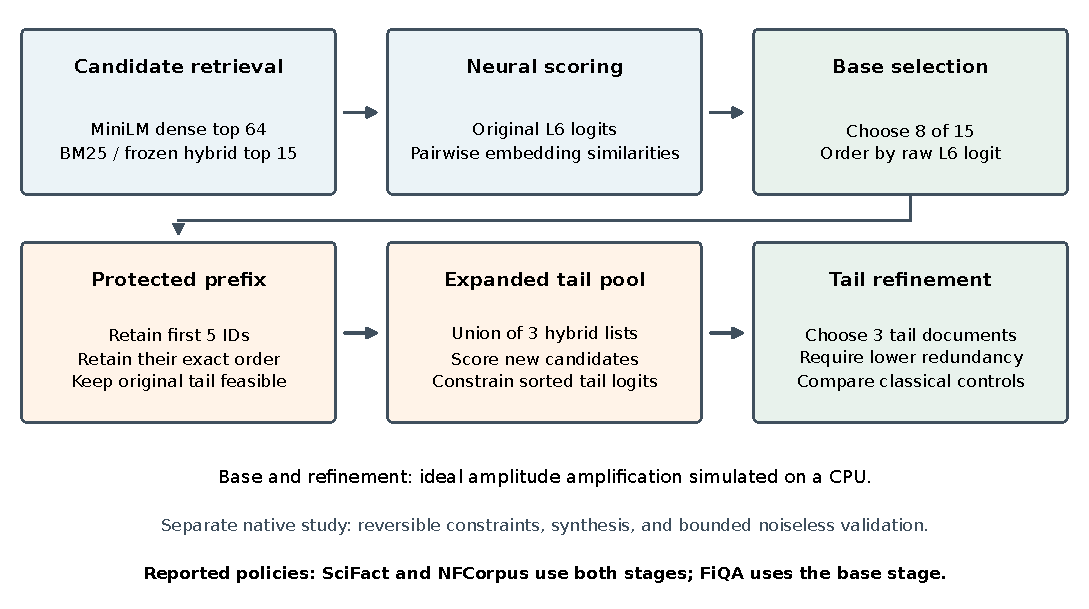
\includegraphics[width=\textwidth]{architecture.pdf}
\caption{System boundaries and reported configurations. Classical retrieval and neural inference precede ideal amplitude amplification simulated on a CPU. The separate native resource study does not replace those classical stages or constitute a full hardware execution of the retrieval pipeline.}
\label{fig:architecture}
\end{figure*}

\subsection{Implementation and measurement boundaries}
Figure~\ref{fig:architecture} distinguishes retrieval, neural relevance inference, base selection, and optional refinement. The application code also supports document ingestion and question-answering interfaces. Their existence does not imply that interface quality, optical character recognition accuracy, or live generated answers were evaluated by these experiments. The measured research pipeline uses public parent-document judgments and frozen passage construction.

The study uses two simulation models. The main selector stores amplitudes for subsets of the required size and constructs their objective values classically. The native study builds reversible circuits with explicit decision and workspace registers. It supplies bounded synthesis and validation evidence; the main selector supplies the retrieval rankings. Neither model includes device routing, noisy execution, or a measured quantum processor.

\section{Relevance-Guided Subset Search}\label{sec:method}
\subsection{Hybrid candidate construction}
The hybrid shortlist is drawn from the dense top-64 pool. Within that pool, let $c_{\max}=\max_i c_i$ and $b_{\max}=\max_i b_i$. The reproduced score is
\begin{equation}
h_i=(1-\beta)\frac{1+c_i}{1+c_{\max}}+\beta\frac{b_i}{b_{\max}}.
\label{eq:hybrid}
\end{equation}
When lexical scores are negligible, only the dense component is used; when its denominator is negligible, that component becomes $(1+c_i)/2$. The numerical tolerance is $10^{-12}$. Hybrid score determines the top-fifteen shortlist, with document ID breaking ties. Thus fusion operates on an already retrieved pool, rather than searching the collection quantum mechanically.

Hybrid scores and dense cosine do not replace the raw cross-encoder logits. For the original fifteen candidates, normalized relevance is
\begin{equation}
r_i=\frac{z_i-z_{\min}}{z_{\max}-z_{\min}},
\label{eq:normalized_relevance}
\end{equation}
with $r_i=0.5$ when the range is negligible. Negative logits are permitted. The normalized values supply optimization coefficients; the final relevance order uses raw logits. Since normalization is local to a shortlist, its values are not calibrated probabilities that can be compared across pools.

\subsection{Base objective and integer encoding}
For $|S|=k=8$, we define base utility as
\begin{equation}
U(S)=\frac{1}{k}\sum_{i\in S}r_i-\lambda\red(S).
\label{eq:base_utility}
\end{equation}
Both terms depend on classical features. Using $A_b=2^8-1=255$, the rounded coefficients are
\begin{align}
a_i&=\operatorname{round}(A_b r_i),\\
a_{ij}&=\operatorname{round}\!\left(\frac{2A_b\lambda}{k-1}d_{ij}\right),\\
E_b(S)&=-\sum_{i\in S}a_i+\sum_{\{i,j\}\subset S}a_{ij}.
\label{eq:base_energy}
\end{align}
Lower integer energy is preferred, and rounding uses ties to even. The raw-L6 top eight initialize the incumbent. Selected outputs are ordered by descending raw logit, with document ID resolving ties.

Without rounding, $-E_b(S)/(A_bk)$ equals~\eqref{eq:base_utility}. Each of the $k$ unary coefficients and $\binom{k}{2}$ pair coefficients has rounding error of at most one half. It follows that
\begin{equation}
\left|\frac{-E_b(S)}{A_bk}-U(S)\right|\leq\frac{k+1}{4A_b}.
\label{eq:base_quantization}
\end{equation}
This bound applies to coefficient approximation for a fixed set. It says nothing about relevance-model error or the gap between utility and judged effectiveness. At $\lambda=0$, the raw-relevance incumbent already maximizes relevance-only utility, so the implementation retains it rather than changing membership when quantized energies tie.

\subsection{Protected-prefix refinement}
Let the seed-specific base ranking be $(s_1,\ldots,s_8)$, its ordered head be $H=(s_1,\ldots,s_5)$, and its original tail be $T_0=\{s_6,s_7,s_8\}$. Construct an expanded candidate union
\begin{equation}
\pool_{\cup}=\bigcup_{\beta\in\{0,0.25,0.5\}}\operatorname{Top}_{15}(h_{\beta};\pool_{64}).
\label{eq:union}
\end{equation}
The union contains the original shortlist and at most 45 parents. We retain the original-shortlist logits and score only newly introduced candidates. This avoids changing the baseline through a different inference-batching context.

The refinement searches $T\subseteq\pool_{\cup}\setminus H$ with $|T|=3$. Sort the tail logits in ascending order, denoted $z_{(1)}(T)\leq z_{(2)}(T)\leq z_{(3)}(T)$. Admissibility requires
\begin{equation}
z_{(j)}(T)\geq z_{(j)}(T_0)-\eps,\quad j\in\{1,2,3\},\quad\eps=10^{-12}.
\label{eq:tail_constraint}
\end{equation}
The constraint compares sorted score values, not document identities: an original tail document may be replaced. Candidates below the smallest permissible score are removed before constructing the subset basis. If $M$ candidates remain, its cardinality basis has $\binom{M}{3}$ states, some of which may still fail the other score conditions.

For fixed thresholds $\theta_j=z_{(j)}(T_0)-\eps$, condition~\eqref{eq:tail_constraint} is equivalently expressed by
\begin{equation}
\sum_{i\in T}\mathbf{1}\{z_i\geq\theta_j\}\geq4-j,\qquad j=1,2,3.
\label{eq:threshold_counts}
\end{equation}
In an ascending tail, the $j$th value reaches $\theta_j$ exactly when at least the largest $4-j$ values reach that threshold. The inclusive comparison handles repeated logits. This count form suits reversible implementation; the sorted form makes admissibility easier to interpret.

The refinement minimizes $\red(H\cup T)$. With $A_r=2^{16}-1$, its integer objective is
\begin{equation}
E_r(H\cup T)=\sum_{\{i,j\}\subset H\cup T}\operatorname{round}(A_r d_{ij}).
\label{eq:refinement_energy}
\end{equation}
Reported redundancy includes head--head, head--tail, and tail--tail terms, even though the head--head contribution is constant during refinement. The oracle marks admissible states whose integer energy is strictly below the incumbent's. The controller accepts a measured update only if true, unrounded redundancy improves by more than $\eps$.

We return the original head in its existing order, followed by the selected tail sorted on raw L6 logits. A high-logit new candidate therefore cannot displace a protected head document. Global union-L6 serves as the control with a different ordering rule.

\subsection{What the constraints guarantee}
\begin{proposition}[Protected ranking metric]\label{prop:prefix}
For fixed query judgments, preserving the first five document IDs and their order preserves nDCG@5 exactly, independently of how the last three outputs are chosen.
\end{proposition}
\begin{IEEEproof}
The numerator of nDCG@5 contains only the gains and discounts at those five ranks. Its ideal denominator is a function of the fixed judgments, not the retrieved tail. Both quantities are unchanged. The equality therefore also holds after seed and query averaging.
\end{IEEEproof}

\begin{proposition}[Incumbent safety]\label{prop:safety}
The original tail is admissible and survives the score prefilter. Every accepted refinement retains eight unique outputs and never increases the reported redundancy relative to its starting base set.
\end{proposition}
\begin{IEEEproof}
Each sorted original-tail score meets its own bound in~\eqref{eq:tail_constraint}, including ties within the tolerance. Its documents therefore survive the smallest-threshold prefilter and supply a cardinality-feasible initial state. The controller replaces that state only with a valid measured tail of size three disjoint from the protected head and with strictly lower true redundancy. Induction over accepted updates proves the claim. If the search ends without improvement, its feasible incumbent is still returned.
\end{IEEEproof}

The set can remain unchanged if the remaining basis is trivial, the incumbent is optimal, or sampling does not find an improvement. The guarantees also leave recall unprotected. An irrelevant candidate can have a higher cross-encoder score and lower pair similarity than a relevant original-tail document. Replacing the latter satisfies the neural-score constraints but reduces the number of judged-relevant outputs. This failure appears in the saved results in Section~\ref{sec:diagnostics}.

For general pair precision $b$, the refinement scale is $A=2^b-1$. Rounding each of the 28 pair coefficients yields
\begin{equation}
\left|\frac{E_r(S)}{28A}-\red(S)\right|\leq\frac{1}{2A}.
\label{eq:refinement_bound}
\end{equation}
For exact integer minimizer $S_A$ and exact float minimizer $S_\star$ over the same admissible domain, applying this inequality twice gives
\begin{equation}
\red(S_A)-\red(S_\star)\leq\frac{1}{A}.
\label{eq:exact_regret}
\end{equation}
The budgeted GAS output need not be the exact encoded optimum. Equation~\eqref{eq:exact_regret} therefore does not bound its search error. At sixteen bits, the per-set approximation bound is about $7.63\times10^{-6}$; greater precision cannot correct a relevance score that misjudges a document.

\subsection{Ideal amplitude amplification and stopping rules}
The base cardinality basis contains $F_b=\binom{15}{8}=6{,}435$ states. Refinement uses $F_r=\binom{M}{3}$ states. Write $|u\rangle=F^{-1/2}\sum_x|x\rangle$ for the uniform state on the corresponding cardinality basis. An oracle and reflection step are
\begin{align}
O_\tau|x\rangle&=(-1)^{[x\text{ admissible}\,\land\,E(x)<\tau]}|x\rangle,\\
G_\tau&=(2|u\rangle\langle u|-I)O_\tau.
\label{eq:amplification}
\end{align}
The compact simulator executes the sign changes and reflection about the mean explicitly, then draws a state according to squared amplitudes. These ideal quantum-search operations run on a classical CPU. The controller does not choose an ideal rotation number from a precomputed optimum or marked-state count.

Each stage starts from a feasible incumbent with sampling window $m=1$. Within the remaining phase budget, a trial draws an integer from zero to $\lceil m\rceil-1$, prepares the uniform state, applies that many steps, and measures. A strict accepted improvement resets the window; otherwise it grows by 1.2 up to $\sqrt F$. For each stage and seed, the recorded limits are 64 phase calls, 32 trials, and a cooperative 15-second time limit. Base and refinement use separate budgets, so a refined request can use up to 128 phase calls.

\begin{table*}[t]
\centering\small
\caption{Refinement controller in implementation order. Integer marking and true-redundancy acceptance have different roles; neither uses test judgments.}
\label{tab:algorithm}
\begin{minipage}{.96\textwidth}
\begin{algorithmic}[1]
\REQUIRE Original ranked eight $B$, expanded scored pool $C$, seed, and recorded stage budgets
\STATE Set $H\gets B[1{:}5]$; $T_0\gets B[6{:}8]$; incumbent $T\gets T_0$; window $m\gets1$
\STATE Preserve original L6 logits; build inclusive score thresholds from $T_0$
\STATE Remove tail candidates below the smallest threshold; enumerate the size-three compact basis
\STATE Construct integer energies and admissibility flags classically for that basis
\WHILE{phase, trial, and cooperative time limits permit another trial}
\STATE Draw a rotation count from the current window, restricted by the remaining phase allowance
\STATE Prepare $|u\rangle$; phase-mark admissible integer improvements; reflect; measure a candidate tail $T'$
\IF{$T'$ is admissible, has lower integer energy, and $\red(H\cup T')<\red(H\cup T)-\eps$}
\STATE Accept $T\gets T'$ and reset $m\gets1$
\ELSE
\STATE Grow $m\gets\min\{1.2m,\sqrt F\}$
\ENDIF
\ENDWHILE
\RETURN Original ordered $H$, followed by $T$ sorted by raw L6 score; retain counts and termination status
\end{algorithmic}
\end{minipage}
\end{table*}

Table~\ref{tab:algorithm} exposes a cost outside the phase-call allowance: the compact simulator evaluates every basis state before amplification. Exact enumeration can inspect that same prepared objective array without simulating amplitudes. A low logical phase count consequently does not establish lower wall-clock work for this selector.

\section{Data and Experimental Protocol}\label{sec:protocol}
\subsection{Collections, splits, and model identities}
Table~\ref{tab:datasets} records the collections, complete judged test-query counts, and frozen base settings. Every positive-query ID in each official test split is evaluated: 300 SciFact, 323 NFCorpus, and 648 FiQA queries. We exclude the partially collected fourth collection. The separate resource study uses saved features from the same domains, not an additional retrieval-effectiveness test.

\begin{table*}[t]
\centering\small
\caption{Recorded datasets and configurations. Documents are parent documents. SciFact development is derived from official training; the other two use official development splits. The lexical weight is $\beta$ and the base redundancy weight is $\lambda$.}
\label{tab:datasets}\begin{tabular}{lrrrrrl}
\toprule
Dataset & Documents & Dev. & Test & $\beta$ & $\lambda$ & Reported policy\\
\midrule
SciFact & 5,183 & 161 & 300 & 0.25 & 0.000 & Base + refinement\\
NFCorpus & 3,633 & 324 & 323 & 0.50 & 0.050 & Base + refinement\\
FiQA & 57,638 & 500 & 648 & 0.00 & 0.025 & Base\\
\bottomrule
\end{tabular}

\end{table*}

The dense encoder, \path{sentence-transformers/all-MiniLM-L6-v2}, produces normalized 384-dimensional vectors. For relevance we use \path{cross-encoder/ms-marco-MiniLM-L6-v2}, with an L2 cross-encoder as the smaller neural control. Repository revisions and model-file hashes in the evidence manifest identify the artifacts used. The journal analysis downloads no new weights and reruns no inference.

We normalize document text with Unicode NFKC and whitespace collapse, using deterministic text handling. Tokenizer offsets are computed without padding or truncation. Chunks contain at most 190 WordPiece content tokens and advance by 158 content tokens; adding two special tokens gives a model input of at most 192 tokens. The maximum query cosine over a parent's chunks becomes its score, with the lowest chunk index breaking an exact tie. We use that original chunk as the representative passage, so methods sharing a pool also share parent IDs and passage representations.

Query lengths must satisfy the content-token limit, and query--passage pairs must satisfy the cross-encoder's 512-token limit; neither check permits silent truncation. The original fifteen logits are retained during expansion so that a different batching context cannot perturb the baseline. Hashes of the corpus, queries, and judgments link the saved inputs to the recorded runs.

\subsection{Development decisions and follow-up status}
For SciFact, the fixed development sample comprises one fifth of the official training queries; NFCorpus and FiQA use their supplied development splits. The base search considers
\begin{equation}
\begin{aligned}
\beta&\in\{0,0.25,0.5\},\\
\lambda&\in\{0,0.01,0.025,0.05\}.
\end{aligned}
\label{eq:development_grids}
\end{equation}
All stochastic settings use seeds zero through four. Eligibility requires mean nDCG@5 and Recall@8 to match or exceed L6-only on the same shortlist within $10^{-12}$. Among eligible settings, the lexicographic order first maximizes nDCG@5, then Recall@8; it then minimizes redundancy, followed by $\lambda$ and finally $\beta$.

SciFact selects a zero diversity weight, which the rule permits. At that setting the relevance-ranked base incumbent already optimizes the unquantized relevance objective. Calling the search GAS does not by itself imply a nonzero diversity effect; the objective, frozen weights, and search procedure have to be interpreted separately.

The L6 MMR grid is 0, 0.1, 0.25, 0.5, 0.75, and 1: six values. The recorded relevance-first preference selects zero diversity weight on these collections. Its measured row represents one operating point, not the complete MMR tradeoff frontier. Cosine-guided controls retain their own frozen settings. Legacy threshold selection considers $\{0.3,0.5,0.7\}$ using development nDCG@5 and the declared tie preferences.

The deterministic 100-query confirmation samples exclude historical development, pilot, and test IDs. The descriptive gate compares refinement with its matched base: mean nDCG@5 must be equal, the mean-recall ratio at least 0.98, and mean redundancy strictly lower. NFCorpus lost 2.1561\% relative recall in confirmation and failed the gate. A recorded decision continued to the full test without changing the method or global gate; the later outcome does not turn the confirmation into a pass.
% TODO(author): Explain how the recall-retention threshold was chosen, if a rationale is documented.

Earlier test outcomes had been observed during development. Although the reported parameters were not retuned against the newer follow-up judgments, those official tests are not an untouched holdout for the redesign. The journal diagnostics retrospectively describe the same saved runs.

\subsection{Controls and comparison fairness}
The original evaluation has twenty methods, with seven expanded-pool policies added for protected-refinement runs. The controls include dense cosine, dense/BM25 RRF with rank constant 60, native cosine and L6 MMR, cosine-guided GAS, L6-only ranking, base L6-guided GAS, greedy and exact optimizers, random search, legacy threshold Grover, and L2/L6 neural models. Cross-encoders on dense fifteen and dense sixty-four use different pools from L6-only on hybrid fifteen.

The seven expanded-pool policies comprise constrained GAS, constrained local-swap greedy, exact float, exact quantized, matched random search, global union-L6 ranking, and union-L6 with the protected prefix. Each constrained policy uses the actual baseline prefix for the seed and the same tail feasibility rules. The random refiner draws $\max(1,2Q)$ uniform subsets in addition to its initial incumbent, with $Q$ denoting the seed's recorded refinement phase count. That matches a declared objective-access allowance, not every operation of the compact simulator.

The exact controls independently enumerate their float or quantized objectives. The GAS controller receives neither their optimum nor the marked-state count. A comparison across pools describes complete policies; one among constrained refiners with identical features isolates their search outcomes for the same objective and admissible domain. These comparisons answer different questions.

\subsection{Metrics, inference, and hardware}
We use nDCG@5, Recall@8, and the redundancy measure in~\eqref{eq:redundancy} as principal metrics; nDCG@8 shows effects at ranks six through eight. Discounted gains use linear judgment values and logarithmic rank discount~\cite{jarvelin2002gain}, and saved rankings are checked with NIST's trec\_eval~\cite{trec_eval}. For a five-seed policy, we first average within each query and then across queries. Seeds do not create independent relevance judgments for a query.

For protected-run inference, the recorded procedure uses 10,000 paired bootstrap resamples with seed zero and 10,000 paired sign-randomization draws with seed one. Differences no larger than $10^{-12}$ are ties. Holm correction covers nine comparators by four metrics per protected dataset. The earlier FiQA nDCG audit covers six declared comparators and removes numerical averaging artifacts before testing. We retain those families and their pointwise intervals rather than choosing a new family to change apparent significance.

The recorded host runs Linux and Python 3.12.3 on an Intel Core i7-1355U with 12 logical CPUs and approximately 15.3\,GiB of RAM. Compute libraries use two threads. Recorded software versions include NumPy 1.26.4, SciPy 1.13.1, CPU PyTorch 2.12.0, Transformers 4.57.6, Sentence Transformers 3.4.1, Qiskit 0.46.0, and Aer 0.13.3~\cite{javadi2024qiskit}. Online latency excludes model loading, corpus/cache restoration, and artificial-query warm-up. Session and host-load records are available, but the experiments were not run in a dedicated latency laboratory.

Online time includes the applicable retrieval, lexical, neural, and selection stages; reused upstream work is charged to each policy that requires it. Base and refinement times are summed for each seeded request before combined selector percentiles are calculated. Request P95 is not divided by the number of seeds. Section~\ref{sec:diagnostics} decomposes mean cost additively, without treating sums of component percentiles as pipeline percentiles.

\section{Recorded Retrieval Results}\label{sec:results}
\subsection{Effectiveness under the declared configurations}
Table~\ref{tab:headline} reports the selected full-test policies. The values come from the completed studies; no new journal experiments were collected. The reported nDCG@5 values are \scifactNdcg{}, \nfcorpusNdcg{}, and \fiqaNdcg{} on SciFact, NFCorpus, and FiQA, respectively. In the first two rows, nDCG@5 is tied to the matched base by prefix preservation. FiQA's row instead reports the earlier fifteen-candidate base selector. The configuration label is therefore necessary to interpret the result.

\begin{table}[t]
\centering\small\setlength{\tabcolsep}{3pt}
\caption{Reported full-test policies. SciFact/NFCorpus include refinement; FiQA uses the earlier base. All quantities within a row come from the same recorded policy.}
\label{tab:headline}\begin{tabular}{lrrrr}
\toprule
Dataset & nDCG@5 & nDCG@8 & Recall@8 & Redundancy $\downarrow$\\
\midrule
SciFact & 0.687833 & 0.698173 & 0.801111 & 0.433636\\
NFCorpus & 0.368865 & 0.346506 & 0.152997 & 0.431771\\
FiQA & 0.357490 & 0.376939 & 0.434063 & 0.531244\\
\bottomrule
\end{tabular}

\end{table}

Relative to matched base selection, SciFact refinement reduces mean redundancy by \scifactRedReduction\% and changes mean Recall@8 by \scifactRecallChange\% relative. NFCorpus reduces redundancy by \nfcorpusRedReduction\% with a +\nfcorpusRecallChange\% relative recall change. The recall changes have different signs across domains. The refinement therefore cannot be described as a general recall improvement, even though the same prefix metric is preserved on both collections.

The FiQA base reaches Recall@8 of \fiqaRecall{} and redundancy of \fiqaRedundancy{}. It matches the reported nDCG@5 and recall of its same-shortlist L6-only control. A later, separately completed 648-query FiQA refinement follow-up preserved nDCG@5 and reduced redundancy by \fiqaFollowupRedReduction\%, but lost \fiqaFollowupRecallLoss\% relative recall. That result failed the frozen 98\% recall-retention gate and was not retuned into a passing result. We retain the prior manuscript's disclosure of this failure without substituting its redundancy value into the earlier base row.

\subsection{Classical and neural comparisons}
Table~\ref{tab:comparators} places the reported policy alongside the declared controls. The cross-encoder shortlist distinctions matter: L6-only uses hybrid fifteen, while the dense-fifteen neural control uses the fifteen highest dense-scoring parents. Differences between those rows include candidate construction. Dense-sixty-four neural reranking additionally exposes the relevance model to more candidates and incurs the corresponding inference cost.

\begin{table*}[t]
\centering\small\setlength{\tabcolsep}{4pt}
\caption{Recorded full-test comparison. n@5 is nDCG@5, R@8 is Recall@8, and Red. is redundancy. Matched search controls use the refined domain on SciFact/NFCorpus and the base domain on FiQA. Additional saved methods remain in the complete CSV export.}
\label{tab:comparators}\begin{tabular}{lrrrrrrrrr}
\toprule
& \multicolumn{3}{c}{SciFact} & \multicolumn{3}{c}{NFCorpus} & \multicolumn{3}{c}{FiQA}\\
Policy & n@5 & R@8 & Red. & n@5 & R@8 & Red. & n@5 & R@8 & Red.\\
\midrule
Dense cosine & 0.6361 & 0.8111 & 0.4756 & 0.3181 & 0.1335 & 0.4398 & 0.3470 & 0.4153 & 0.5363\\
Dense/BM25 RRF & 0.6677 & 0.8149 & 0.4727 & 0.3491 & 0.1394 & 0.4394 & 0.3509 & 0.4262 & 0.5327\\
Legacy threshold Grover & 0.6364 & 0.8111 & 0.4756 & 0.3181 & 0.1334 & 0.4398 & 0.3458 & 0.4150 & 0.5363\\
Cosine-guided GAS & 0.6311 & 0.7742 & 0.4490 & 0.3160 & 0.1235 & 0.3996 & 0.3452 & 0.4093 & 0.5215\\
L6 relevance only & 0.6878 & 0.8086 & 0.4480 & 0.3689 & 0.1500 & 0.4447 & 0.3575 & 0.4341 & 0.5313\\
L6 MMR & 0.6878 & 0.8086 & 0.4480 & 0.3689 & 0.1500 & 0.4447 & 0.3575 & 0.4341 & 0.5313\\
Base L6-guided GAS & 0.6878 & 0.8086 & 0.4480 & 0.3689 & 0.1501 & 0.4434 & 0.3575 & 0.4341 & 0.5312\\
Matched greedy & 0.6878 & 0.8011 & 0.4336 & 0.3689 & 0.1530 & 0.4318 & 0.3575 & 0.4341 & 0.5311\\
Matched exact float & 0.6878 & 0.8011 & 0.4336 & 0.3689 & 0.1530 & 0.4318 & 0.3575 & 0.4343 & 0.5309\\
Matched exact integer & 0.6878 & 0.8011 & 0.4336 & 0.3689 & 0.1530 & 0.4318 & 0.3575 & 0.4341 & 0.5311\\
Matched random & 0.6878 & 0.8011 & 0.4338 & 0.3689 & 0.1531 & 0.4320 & 0.3575 & 0.4341 & 0.5313\\
L2, dense 15 & 0.6431 & 0.8049 & 0.4642 & 0.3509 & 0.1396 & 0.4486 & 0.3319 & 0.4217 & 0.5295\\
L6, dense 15 & 0.6790 & 0.8104 & 0.4655 & 0.3621 & 0.1423 & 0.4537 & 0.3575 & 0.4341 & 0.5313\\
L2, dense 64 & 0.6321 & 0.7916 & 0.4329 & 0.3481 & 0.1438 & 0.4468 & 0.2973 & 0.3918 & 0.4962\\
L6, dense 64 & 0.6815 & 0.8087 & 0.4379 & 0.3670 & 0.1437 & 0.4586 & 0.3535 & 0.4160 & 0.5033\\
Reported GAS policy & 0.6878 & 0.8011 & 0.4336 & 0.3689 & 0.1530 & 0.4318 & 0.3575 & 0.4341 & 0.5312\\
\bottomrule
\end{tabular}

\end{table*}

Matched greedy and exact-float refiners have the same aggregate nDCG@5, nDCG@8, Recall@8, and redundancy as constrained GAS on the SciFact and NFCorpus tests. This agreement shows that the measured quality of those outputs does not depend on the Grover search mechanism. The constrained objective and the available candidates explain a benefit that several optimizers can realize.

Table~\ref{tab:expanded} further separates candidate expansion, prefix retention, and constrained set optimization. Global union-L6 permits complete reordering. Protected-prefix union-L6 preserves the head but chooses the tail by neural relevance. The constrained optimizers additionally optimize pair redundancy under the score thresholds. These controls address different sources of change; grouping them under one generic ``reranking'' label would obscure the mechanism being evaluated.

\begin{table*}[t]
\centering\small\setlength{\tabcolsep}{4pt}
\caption{Expanded-pool controls on the two protected-refinement test runs. All four metrics are shown to expose tail effects hidden by a fixed top five. FiQA has no corresponding expanded-pool headline in the selected source mapping.}
\label{tab:expanded}\begin{tabular}{lrrrrrrrr}
\toprule
& \multicolumn{4}{c}{SciFact} & \multicolumn{4}{c}{NFCorpus}\\
Policy & n@5 & n@8 & R@8 & Red. & n@5 & n@8 & R@8 & Red.\\
\midrule
Union L6, global order & 0.6860 & 0.6972 & 0.8037 & 0.4475 & 0.3688 & 0.3472 & 0.1522 & 0.4477\\
Union L6, protected prefix & 0.6878 & 0.6993 & 0.8037 & 0.4474 & 0.3689 & 0.3466 & 0.1523 & 0.4474\\
Constrained GAS & 0.6878 & 0.6982 & 0.8011 & 0.4336 & 0.3689 & 0.3465 & 0.1530 & 0.4318\\
Constrained greedy & 0.6878 & 0.6982 & 0.8011 & 0.4336 & 0.3689 & 0.3465 & 0.1530 & 0.4318\\
Constrained exact float & 0.6878 & 0.6982 & 0.8011 & 0.4336 & 0.3689 & 0.3465 & 0.1530 & 0.4318\\
Constrained exact integer & 0.6878 & 0.6982 & 0.8011 & 0.4336 & 0.3689 & 0.3465 & 0.1530 & 0.4318\\
Constrained random & 0.6878 & 0.6982 & 0.8011 & 0.4338 & 0.3689 & 0.3468 & 0.1531 & 0.4320\\
\bottomrule
\end{tabular}

\end{table*}

The observed tradeoffs are visualized in Fig.~\ref{fig:tradeoffs}. Some inexpensive or less relevance-focused policies have lower redundancy while also having lower recall. The graph contains measured operating points, not a tuned Pareto frontier or a proof of dominance over every possible setting. In particular, the zero-diversity MMR point does not represent the complete range of MMR operating choices.

\begin{figure*}[t]
\centering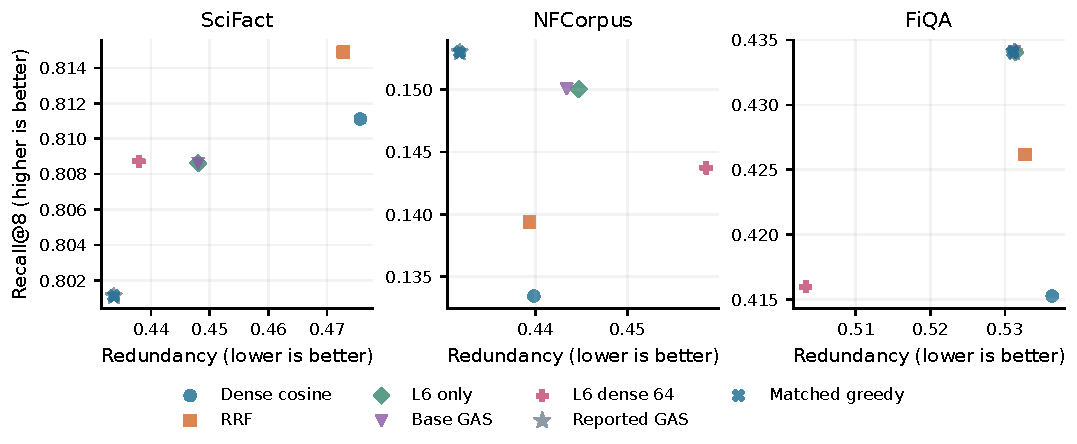
\includegraphics[width=\textwidth]{observed_tradeoffs.pdf}
\caption{Observed Recall@8--redundancy operating points from the saved runs. Coincident points can arise when policies return the same effective outputs. Candidate pools differ as specified in the protocol; the graph is descriptive and does not imply matched causal comparisons across every point.}
\label{fig:tradeoffs}
\end{figure*}

\subsection{Paired uncertainty and interpretation}
Table~\ref{tab:statistics} reproduces paired differences against the base for the protected datasets. SciFact's recall interval includes both a loss and a gain, while its mean is negative. NFCorpus's positive recall interval is pointwise; the recorded raw probability does not produce a rejection after the complete Holm family is considered. The distinction between a displayed interval and a familywise testing decision must remain explicit.

\begin{table*}[t]
\centering\small
\caption{Recorded paired inference: reported refinement minus base on SciFact/NFCorpus. $\dagger$FiQA is its earlier base minus L6-only for the independently audited nDCG@5 comparison. Intervals are pointwise, not simultaneous; Holm decisions use each original full family.}
\label{tab:statistics}\begin{tabular}{llrrrc}
\toprule
Dataset & Metric & Mean difference & Paired 95\% CI & Raw $p$ & Holm reject\\
\midrule
SciFact & nDCG@5 & +0.00000 & [+0.00000, +0.00000] & 1.00000 & No\\
SciFact & nDCG@8 & -0.00268 & [-0.00811, +0.00231] & 0.30427 & No\\
SciFact & Recall@8 & -0.00750 & [-0.02417, +0.00750] & 0.45645 & No\\
SciFact & Redundancy & -0.01439 & [-0.01680, -0.01216] & 0.00010 & Yes\\
NFCorpus & nDCG@5 & +0.00000 & [+0.00000, +0.00000] & 1.00000 & No\\
NFCorpus & nDCG@8 & +0.00094 & [-0.00248, +0.00445] & 0.58974 & No\\
NFCorpus & Recall@8 & +0.00293 & [+0.00038, +0.00622] & 0.03690 & No\\
NFCorpus & Redundancy & -0.01165 & [-0.01405, -0.00938] & 0.00010 & Yes\\
FiQA & nDCG@5$^\dagger$ & 0.00000 & [0.00000, 0.00000] & 1.00000 & No\\
\bottomrule
\end{tabular}

\end{table*}

The empirical 98\% mean-recall gate is not a statistical noninferiority test, and an interval containing zero does not establish equivalence. Stronger inferential claims would require a justified noninferiority margin, a prospective analysis, and data whose role in method development is appropriately controlled. The present evidence supports the recorded descriptive gate outcomes and the stated paired comparisons.

The FiQA statistical audit also illustrates why floating-point conventions matter. Averaging five identical seeded scores can produce a difference of approximately one unit in the last place relative to a deterministic control. A significance test must not promote that numerical artifact into evidence of a retrieval improvement. The recorded $10^{-12}$ tie policy addresses this problem while leaving rankings and reported raw means intact.

\subsection{Latency and optimization outcomes}
Complete online median and P95 times appear in Table~\ref{tab:latency}. Expanded-pool inference increases complete latency relative to the matched base. A small refinement time does not make the two-stage pipeline equally inexpensive. Comparisons with dense-sixty-four rerankers involve both cost and candidate opportunity and should not be reduced to a universal speed claim.

\begin{table*}[t]
\centering\small\setlength{\tabcolsep}{6pt}
\caption{Composed online latency, milliseconds per seeded request. Values include all applicable upstream stages. P50/P95 are computed over recorded request totals; restoration, model loading, and warm-up are separate.}
\label{tab:latency}\begin{tabular}{lrrrrrr}
\toprule
& \multicolumn{2}{c}{SciFact} & \multicolumn{2}{c}{NFCorpus} & \multicolumn{2}{c}{FiQA}\\
Policy & P50 & P95 & P50 & P95 & P50 & P95\\
\midrule
Dense cosine & 33.3 & 48.3 & 24.5 & 32.9 & 79.9 & 98.5\\
Dense/BM25 RRF & 61.6 & 94.9 & 31.0 & 44.5 & 225.3 & 328.3\\
Legacy threshold Grover & 38.2 & 313.6 & 25.2 & 281.6 & 84.3 & 231.9\\
Cosine-guided GAS & 42.3 & 56.8 & 33.7 & 42.0 & 84.1 & 102.5\\
L6 relevance only & 955.3 & 1085.4 & 851.9 & 901.4 & 650.0 & 821.1\\
L6 MMR & 955.5 & 1085.7 & 852.1 & 901.6 & 650.1 & 821.3\\
Base L6-guided GAS & 963.2 & 1093.7 & 859.8 & 909.1 & 653.8 & 826.7\\
Matched greedy & 1405.4 & 1670.7 & 1145.5 & 1479.6 & 650.0 & 821.2\\
Matched exact float & 1405.2 & 1670.6 & 1145.3 & 1479.3 & 651.2 & 822.5\\
Matched exact integer & 1405.2 & 1670.6 & 1145.3 & 1479.3 & 651.1 & 822.4\\
Matched random & 1405.2 & 1670.6 & 1145.4 & 1479.3 & 651.9 & 824.8\\
L2, dense 15 & 348.0 & 403.0 & 310.5 & 331.5 & 238.9 & 294.6\\
L6, dense 15 & 915.8 & 1029.2 & 832.5 & 882.5 & 539.6 & 618.2\\
L2, dense 64 & 1374.7 & 1562.5 & 1242.5 & 1319.6 & 763.7 & 912.2\\
L6, dense 64 & 3799.0 & 4322.2 & 3460.8 & 3630.9 & 2037.9 & 2437.9\\
Reported GAS policy & 1406.5 & 1672.3 & 1146.8 & 1481.3 & 653.8 & 826.7\\
\bottomrule
\end{tabular}

\end{table*}

Table~\ref{tab:search} distinguishes logical work from outcome quality. An exact objective hit is evaluated against the corresponding exact float-redundancy optimum for refinement and the exact integer optimum for the base. Such a hit certifies neither maximum judged recall nor maximum nDCG. Budget exhaustion, a trivial basis, and an unchanged incumbent are meaningful outcomes retained in the request denominator.

\begin{table*}[t]
\centering\small
\caption{Recorded search work and combined selector latency in milliseconds. The first phase column counts inherited base work for refined policies; it is zero for base-only FiQA. The next column counts the current stage. Optimum-hit definitions follow the text.}
\label{tab:search}\begin{tabular}{lrrrrrr}
\toprule
Dataset & Requests & Base phases & Refine/base phases & Optimum-hit rate & Selector P50 & Selector P95\\
\midrule
SciFact & 1500 & 64.00 & 20.08 & 1.000 & 9.66 & 10.67\\
NFCorpus & 1615 & 63.91 & 17.82 & 1.000 & 9.49 & 11.02\\
FiQA & 3240 & 0.00 & 64.00 & 0.994 & 3.95 & 4.54\\
\bottomrule
\end{tabular}

\end{table*}

The work counts document this implementation's behavior. They cannot establish physical acceleration: the CPU simulator prepares the complete objective array, and classical methods can inspect that array directly. The objective assumptions and measured cost boundaries remain explicit.

\section{Journal Extension: Coverage, Failure, and Cost Diagnostics}\label{sec:diagnostics}
\subsection{Candidate coverage separates retrieval from selection}
Saved feature and ranking records let us reconstruct candidate membership and evaluate~\eqref{eq:coverage_ceiling} for dense sixty-four, hybrid fifteen, and the expanded union where available. We check pool sizes, subset inclusion, and parent IDs independently of historical field names before computing coverage. No new rankings are created.

\begin{table*}[t]
\centering\small
\caption{New secondary analysis of saved candidate pools. Judged coverage includes every positively judged parent in the pool. The Recall@8 ceiling additionally enforces the eight-output budget and relaxes relevance-score and prefix constraints. Values are query means.}
\label{tab:coverage}\begin{tabular}{llrrr}
\toprule
Dataset & Pool & Mean size & Judged coverage & Recall@8 ceiling\\
\midrule
SciFact & Dense 64 & 64.00 & 0.9243 & 0.9243\\
SciFact & Hybrid 15 & 15.00 & 0.8569 & 0.8569\\
SciFact & Expanded union & 22.30 & 0.8903 & 0.8903\\
NFCorpus & Dense 64 & 64.00 & 0.2666 & 0.2375\\
NFCorpus & Hybrid 15 & 15.00 & 0.1780 & 0.1725\\
NFCorpus & Expanded union & 20.29 & 0.2028 & 0.1942\\
FiQA & Dense 64 & 64.00 & 0.6489 & 0.6483\\
FiQA & Hybrid 15 & 15.00 & 0.4824 & 0.4824\\
\bottomrule
\end{tabular}

\end{table*}

Table~\ref{tab:coverage} and Fig.~\ref{fig:coverage} show how much candidate opportunity differs by collection. SciFact's ceiling is \scifactShortCeiling{} for hybrid fifteen and \scifactUnionCeiling{} for the expanded union. The corresponding NFCorpus ceilings are \nfcorpusShortCeiling{} and \nfcorpusUnionCeiling{}. FiQA's base shortlist has a ceiling of \fiqaShortCeiling{}, compared with \fiqaDenseCeiling{} for dense sixty-four. These are optimistic opportunities under the judgments, not predictions of a learned reranker's performance.

For \scifactNoRelevant{} SciFact, \nfcorpusNoRelevant{} NFCorpus, and \fiqaNoRelevant{} FiQA queries, the hybrid shortlist contains no positively judged parent. An eight-of-fifteen selector cannot improve judged recall on those queries without different candidates. Expansion recovers some exclusions in the protected datasets, but stays inside dense sixty-four and cannot recover a corpus document missing from that set.

\begin{figure*}[t]
\centering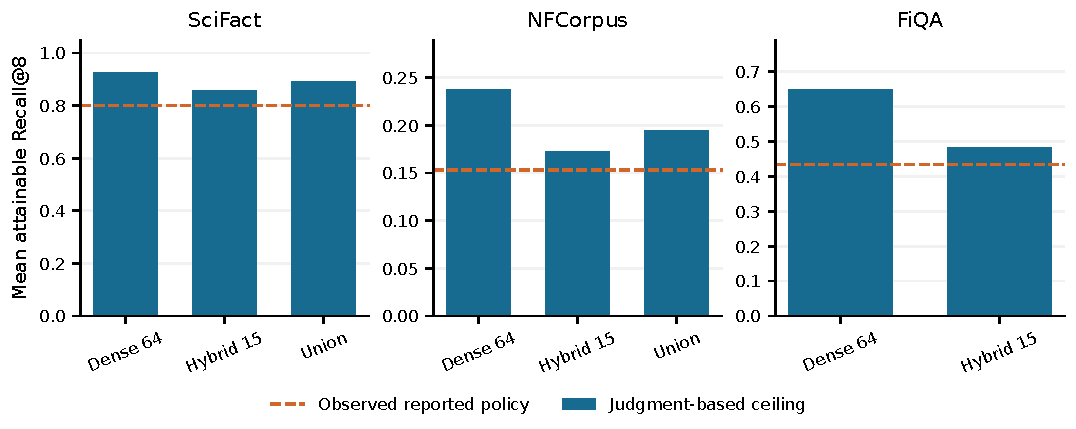
\includegraphics[width=\textwidth]{candidate_coverage.pdf}
\caption{New judgment-based Recall@8 ceilings for the saved candidate pools, compared with the observed reported-policy recall. The dashed line is the same policy within each dataset panel. Expanded-union ceilings relax the protected-prefix and tail-score constraints and therefore do not measure pure search inefficiency.}
\label{fig:coverage}
\end{figure*}

The number of judged-relevant documents also changes the scale of Recall@8. Even eight perfect outputs recover only a fraction of a large relevant set. NFCorpus contains queries with substantially larger relevant sets than the single-evidence cases common in SciFact; its lower recall reflects task structure as well as candidate opportunity and ranking performance. Comparing policies on the same queries, against the relevant candidate ceiling, helps separate these factors.

The union widens the relaxed opportunity set, but the actual task commits five positions to the original head and requires replacements to satisfy neural-score dominance. Redundancy remains a proxy for complementary evidence. The gap to the union ceiling therefore reflects constraints and model errors as well as the finite search budget.

\subsection{Mean improvements coexist with individual losses}
Table~\ref{tab:query_outcomes} counts changes from the reference policy after seed averaging within each query. Against base GAS, SciFact has \scifactWins{} recall gains, \scifactLosses{} losses, and \scifactTies{} ties; NFCorpus has \nfcorpusWins{} gains, \nfcorpusLosses{} losses, and \nfcorpusTies{} ties. The favorable NFCorpus mean thus includes queries that lose recall. FiQA has no recall changes beyond the tie tolerance against L6-only, although some memberships and redundancy values differ.

\begin{table*}[t]
\centering\small\setlength{\tabcolsep}{4pt}
\caption{New query-level outcome and seed-stability analysis. References are base GAS for SciFact/NFCorpus and L6-only for FiQA. Counts use a $10^{-12}$ numerical tie tolerance. Seed-varying ranks count queries with more than one final ordered list among the five saved seeds.}
\label{tab:query_outcomes}\begin{tabular}{lrrrrrr}
\toprule
Dataset & Recall wins & Ties & Losses & Lower redundancy & Seed-varying ranks & Seed-varying recall\\
\midrule
SciFact & 2 & 293 & 5 & 158 & 0 & 0\\
NFCorpus & 15 & 295 & 13 & 135 & 29 & 3\\
FiQA & 0 & 648 & 0 & 6 & 7 & 0\\
\bottomrule
\end{tabular}

\end{table*}

Redundancy falls for \scifactLowerRed{} SciFact queries and \nfcorpusLowerRed{} NFCorpus queries, and rises for none, consistent with Proposition~\ref{prop:safety}. The paired changes in Fig.~\ref{fig:paired} show many zeros and a small subset with recall differences. A mean does not show how those outcomes are distributed.

\begin{figure*}[t]
\centering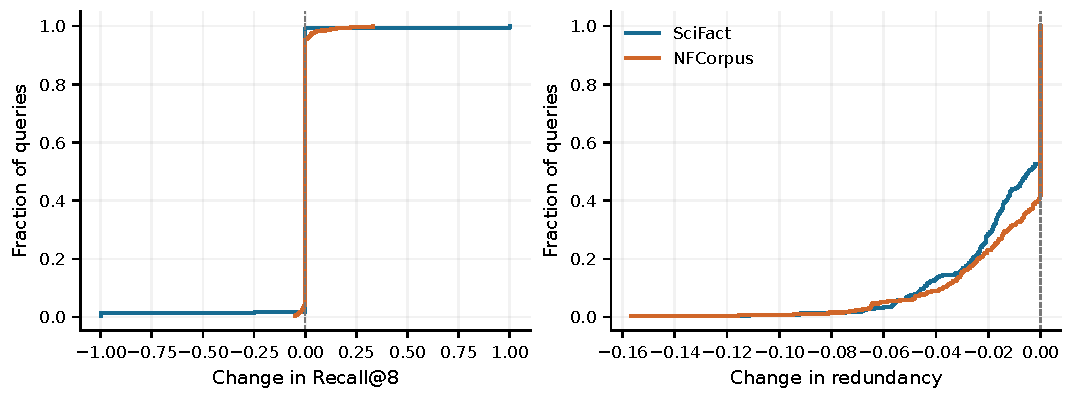
\includegraphics[width=\textwidth]{paired_distributions.pdf}
\caption{New empirical cumulative distributions of query-level refinement-minus-base differences. Recall changes can be positive or negative. Nonpositive redundancy changes follow the refinement acceptance rule. Seeds are averaged within queries before these distributions are constructed.}
\label{fig:paired}
\end{figure*}

The following extreme cases were chosen deterministically to illustrate the risk, not to represent the full test set. SciFact query 384 has one positively judged relevant parent. Base recall is 1 and refined recall is 0, although the candidate-pool ceiling is 1 and the top five are unchanged. The only relevant output was lost below the protected head. Redundancy fell by approximately 0.04373 even as judged retrieval worsened.

For NFCorpus query PLAIN-2570, the judgments contain 40 relevant parents. Base Recall@8 is 0.075 and refined Recall@8 is 0.025, or three versus one positively judged output. Mean redundancy falls by approximately 0.09454, while the relaxed Recall@8 ceiling is 0.125 for both the original and expanded pools. Candidate opportunity alone does not explain the loss; admissibility, relevance estimates, and the objective also matter. The fixed retrospective selection rule used lowest paired recall change, then largest redundancy decrease, then query ID.

Protecting a top-five metric can serve an application that values that prefix, but it does not establish that the remaining evidence can be replaced safely. A mean-retention threshold may hide a severe loss on an individual query. Recall distributions, the number of harmed queries, and their application-specific costs should accompany the mean.

\subsection{Seed stability is a property of outputs, not independent evidence}
Across seeds, final rankings differ on \scifactSeedVary{} SciFact, \nfcorpusSeedVary{} NFCorpus, and \fiqaSeedVary{} FiQA queries. Recall varies on \scifactSeedRecall{}, \nfcorpusSeedRecall{}, and \fiqaSeedRecall{} queries, respectively. Different sampled trajectories can lead to the same final output; the five-seed average does not by itself describe that distinction.

Stable outputs do not create independent queries, and different tail documents can share a judged status without changing recall. On NFCorpus, more queries have varying ordered lists than varying recall. The complete seed export retains scores and search statuses, allowing this difference to be inspected directly rather than inferred from aggregate variance.

When stochastic search repeatedly reaches an output also found by matched greedy and exact methods, the result does not identify randomness or amplitude amplification as the unique cause of the effectiveness gain. It does describe this implementation's stability under the recorded budgets and seeds.

\subsection{Additive cost attribution and the scope for selector acceleration}
For each primary seeded request, the journal exporter reconstructs
\begin{align}
T_{\mathrm{online}}={}&T_{\mathrm{upstream}}+T_{\mathrm{L6,original}}
+T_{\mathrm{L6,extra}}\nonumber\\
&+T_{\mathrm{base}}+T_{\mathrm{refine}}.
\label{eq:cost_composition}
\end{align}
Upstream time covers query encoding, dense search, representative features, and applicable lexical/hybrid/union processing. Extra inference and refinement are zero for the FiQA base. We check each sum against the saved request total before taking means. Composed stage measurements are additive; separately measured percentiles are not necessarily so.

\begin{figure*}[t]
\centering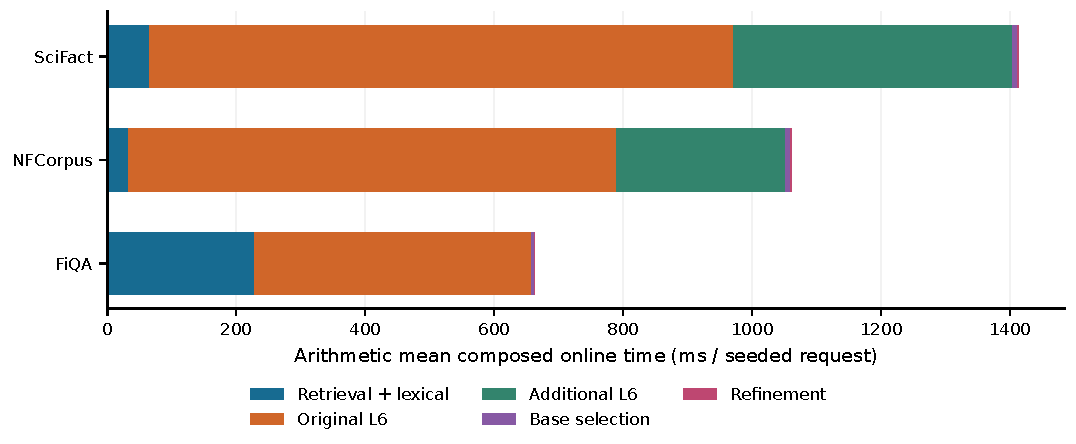
\includegraphics[width=\textwidth]{cost_decomposition.pdf}
\caption{New decomposition of arithmetic mean online time using additive per-request components. Small selector segments are retained. The plot uses means for additivity; Table~\ref{tab:latency} separately reports request-level medians and P95 values. Differences between collection sessions are not controlled cross-session speed experiments.}
\label{fig:cost}
\end{figure*}

In Fig.~\ref{fig:cost}, original L6 inference accounts for \scifactOriginalLsixShare\%, \nfcorpusOriginalLsixShare\%, and \fiqaOriginalLsixShare\% of the respective primary mean online times. Additional L6 scoring further dominates the refined pipelines. Base-plus-refinement selection accounts for \scifactSelectorShare\%, \nfcorpusSelectorShare\%, and \fiqaSelectorShare\%, respectively. Even an idealized removal of all measured selector time would leave most of the composed request cost.

For $f=\overline{T}_{\mathrm{selector}}/\overline{T}_{\mathrm{online}}$, a hypothetical zero-time selector with unchanged upstream stages could reduce the mean by fraction $f$. The idealized speedup would be $1/(1-f)$. This bound accounts for the same staged computation; it is not a hardware prediction. A practical quantum implementation would still need state preparation, data access, reversible arithmetic, and measurement. Within the measured cost boundary, reduced selection phase counts alone give little support to an end-to-end acceleration claim.

\section{Recorded Resource Study and Precision Sensitivity}\label{sec:resources}
\subsection{Compact simulation and native circuits solve different accounting tasks}
The compact selector represents only fixed-cardinality subsets. Its complex128 amplitude array uses $16F$ bytes, where $F=\binom{15}{8}$ for the base or $F=\binom{M}{3}$ for refinement. This allocation excludes stored coefficients, energies, candidate features, and process memory. A full $\nu$-qubit statevector would instead require $16\,2^\nu$ bytes for amplitudes alone. Neither expression measures total system memory.

Compact simulation enumerates basis energies before amplification, so its objective evaluations must be counted separately from incumbent checks, measured trials, and logical phase calls. The recorded convention assigns two reversible objective calls to a phase operation for compute and uncompute. Constraint evaluation, state preparation, reflection, and physical data access would add work to an actual circuit execution. A logical query count does not capture all of these costs.

The native study uses 32 saved training queries per collection, drawn from the confirmation samples. It evaluates five compact-search seeds, tail pools of 3, 5, 8, 12, 16, or 20 candidates, and pair precisions of 4, 8, 12, or 16 bits. Its 178 completed tasks include 80 native synthesis cells. Actual pool availability is retained: a requested size unavailable for a real query is not silently replaced by a smaller pool. Artificial stress instances at the specified larger sizes are labeled separately.

The study was completed before this journal manuscript. It provides neither new relevance judgments nor another full-test evaluation. Its controlled subpools retain the original tail, and native representatives are the first two eligible frozen seed-zero queries for a dataset/pool, when available. The representatives remain fixed across precisions. Comparisons across pool sizes may nevertheless involve different eligible queries, so growth curves describe the measured cells rather than a random population scaling law.

\subsection{Reversible constraint and objective registers}
Writing $x_i\in\{0,1\}$ for a remaining tail candidate, the integer refinement objective has the polynomial form
\begin{equation}
E(x)=C_H+\sum_i\alpha_i x_i+\sum_{i<j}\alpha_{ij}x_ix_j,
\label{eq:native_polynomial}
\end{equation}
where $C_H$ contains fixed head--head terms, $\alpha_i$ sums rounded head--candidate terms, and $\alpha_{ij}$ represents a rounded candidate pair. The oracle evaluates signed improvement relative to the incumbent and marks only states with cardinality three and all three threshold-count conditions in~\eqref{eq:threshold_counts}.

The register allocation comprises $M$ decision qubits, $w$ signed-value qubits, $c=\lceil\log_2(M+1)\rceil$ counter qubits, $c-1$ comparator workspace qubits, and four constraint flags. Thus,
\begin{equation}
\nu=M+w+2c+3.
\label{eq:logical_width}
\end{equation}
The signed width must bound the objective difference on all bit strings, including states with invalid cardinality. Designing $w$ from valid three-element subsets alone could permit overflow on states the circuit must process before rejecting them. The implementation bounds the full polynomial domain and includes every workspace register in the reported total.

The oracle computes objective and constraints, conditionally applies the phase, and reverses the computation. The same counter and comparison workspace can be reused for successive threshold checks, while their flags are retained until phase marking. This structure explains both the logical-width formula and why a compact classical basis dimension is not an interchangeable qubit count.

\begin{table}[t]
\centering\small\setlength{\tabcolsep}{3pt}
\caption{Recorded native-oracle synthesis summary. Slash-separated entries compare 4/16-bit coefficients; full four-precision measurements are retained in the accompanying native CSV. Width includes workspace. Depth and CX values are maxima over the stated bounded sample; stress rows are artificial.}
\label{tab:native}\begin{tabular}{rlrrr}
\toprule
Tail & Source & Qubits & Depth & CX gates\\
\midrule
3 & real & 19/31 & 1049/1865 & 992/2408\\
5 & real & 23/35 & 3891/5955 & 3256/6160\\
8 & real & 29/41 & 15067/20722 & 11684/18240\\
12 & real & 34/46 & 27570/41294 & 22068/36076\\
16 & stress & 39/51 & 61665/67687 & 43628/52212\\
20 & stress & 43/55 & 79769/96137 & 58220/75556\\
\bottomrule
\end{tabular}

\end{table}

Table~\ref{tab:native} summarizes the measured cells. Figure~\ref{fig:native} includes all four precision levels and distinguishes real samples from artificial stress cases. Synthesis uses the unrestricted $u,\mathrm{cx}$ basis, optimization level one, and transpiler seed zero. These are logical resources without coupling-map routing, device calibration, or error correction. The gate count therefore cannot be described as the cost of execution on a particular processor.

\begin{figure*}[t]
\centering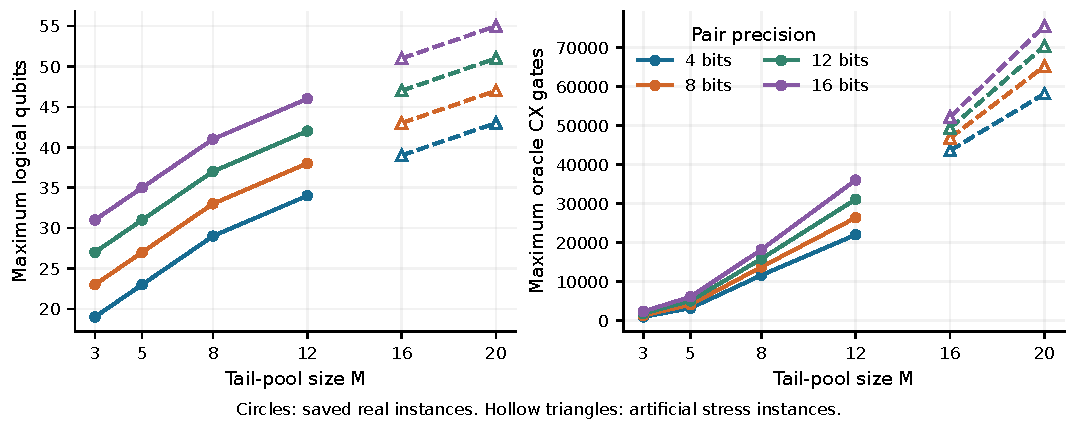
\includegraphics[width=\textwidth]{native_resources.pdf}
\caption{All recorded precision levels for native logical width and oracle CX count. Real-instance points summarize the available fixed representatives; hollow triangles are artificial stress cells. Connecting lines aid inspection and are not fitted scaling models.}
\label{fig:native}
\end{figure*}

\subsection{Precision and search error}
The coefficient bound in~\eqref{eq:refinement_bound} decreases with $b$. The observed GAS output can nevertheless have a larger gap to the exact float optimum because a finite search budget need not find the exact integer optimum. Figure~\ref{fig:precision} separates this empirical search outcome from a statement about coefficient approximation. The saved float gap is the output redundancy minus the exact admissible float optimum for that instance; the quantized gap uses the exact encoded optimum.

\begin{figure*}[t]
\centering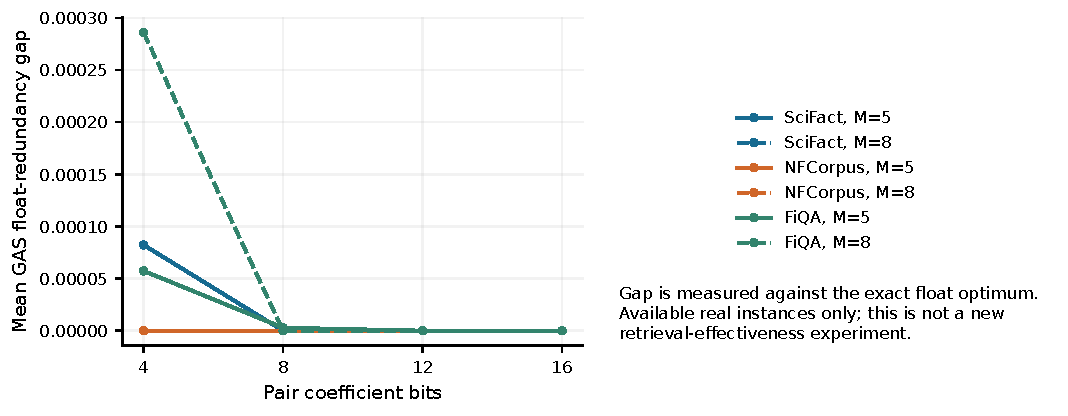
\includegraphics[width=\textwidth]{precision_gaps.pdf}
\caption{Recorded GAS float-redundancy gaps across pair precision for available real five- and eight-candidate subpools. Values are means over the study's fixed available requests, not new retrieval runs. Search error can dominate coefficient error; the exact-optimizer regret bound does not bound these GAS curves.}
\label{fig:precision}
\end{figure*}

Greater precision may distinguish more objective values while increasing signed arithmetic width and circuit work. It does not necessarily yield a monotone improvement in a stochastic, budget-limited output. Nor does a smaller optimization gap imply improved judged relevance: the objective still penalizes pair similarity subject to estimated-score constraints. This is why the primary paper reports retrieval metrics, exact objective controls, and resources together.

\subsection{Validation coverage and explicit limits}
Complete-iteration synthesis, including generic fixed-weight preparation and reflection, is limited to at most eight decision qubits. Native validation simulation is limited to at most five decisions. Six complete iterations passed phase-sensitive validation; 42 other simulation attempts were refused by the conservative memory guard. These refusals mark the limits of the simulations; they do not demonstrate successful execution of larger circuits. Separate small two-bit toy checks exercise nontrivial five-decision marking and reflection.

The native simulator uses a noiseless matrix-product-state method with zero configurable truncation threshold, maximum bond dimension 128, and a $10^{-8}$ probability tolerance. An independently constructed expected-state inverse followed by local $Z$ expectations bounds state mismatch and workspace leakage. Every circuit worker has 120-second and 2\,GiB limits. Larger native simulations, a noise sweep, hardware routing, and physical execution remain unperformed.

Construction, transpilation, native validation, compact selection, allocation profiling, and complete-pipeline timing have different boundaries. Per-method allocation profiling is a separate replay excluded from selector timing, while the fresh worker's process RSS covers its complete grid. Keeping these boundaries separate prevents an allocation replay from inflating one reported time while a costly prerequisite disappears from another.

\section{Discussion, Limitations, and Reproducibility}\label{sec:discussion}
\subsection{What the combined evidence establishes}
The results are consistent with an interpretation based on constrained selection. Protecting a ranking prefix produces a deterministic guarantee for the corresponding truncated ranking metric. Optimizing the tail lowers the declared pair-similarity measure for many queries, but the effect on relevance depends on errors in the neural score model and on the available candidates. The coverage and loss-distribution analyses help explain how these outcomes can occur together.

Classical-control agreement changes the appropriate attribution of the result. If constrained greedy and exact selection reach the same aggregate quality as GAS, the gain over base selection belongs to the shared candidate/objective/constraint policy. The data do not identify an extra effectiveness contribution from amplitude amplification. The small constrained domains also make exact controls practical, which is precisely why excluding them would leave the central claim weakly tested.

The cost decomposition also limits the efficiency claim: selector arithmetic accounts for a small part of the complete pipeline, while neural relevance inference accounts for a substantial share. An optimization strategy intended to improve application latency should therefore account for candidate scoring and upstream work, rather than optimize an isolated phase-query count and assume a comparable end-to-end gain. This conclusion is specific to the recorded pipeline and host; a substantially different access model would require its own measurements.

\subsection{Construct and measurement validity}
Redundancy in this article is a clipped embedding-similarity average. It does not directly measure repeated facts, semantic contradiction, evidence complementarity, or answer faithfulness. Correlated but necessary evidence can receive a high penalty. Dissimilar irrelevant text can receive a low penalty. A future application-level study should test whether a chosen reduction in this proxy improves the outcomes that motivate selection in the first place.

Parent-document judgments and representative passages introduce another boundary. A relevant parent may contain information outside its highest-cosine chunk, and a cross-encoder score on one representative passage may not reflect the full parent. Dense top-64 filtering, hybrid top-fifteen filtering, and score-dominance constraints can each remove useful opportunities. The journal's judgment-based ceilings reveal some of those losses, but incomplete judgments prevent treating them as ceilings on all human relevance.

Preserving nDCG@5 does not preserve every aspect of retrieval quality. Recall@8 and nDCG@8 can change, individual queries can lose substantial recall, and the tail may be used by a downstream consumer despite its lower rank. Similarly, a descriptive mean-retention gate is weaker than a prospective statistical noninferiority design. The observed failures are therefore material to the interpretation, not exceptions that can be omitted from a favorable summary.

\subsection{Internal and external validity}
The official tests were reused during the research trajectory. Recorded follow-up settings were not retuned on their outcomes, but prior observation limits confirmatory interpretation. NFCorpus's failed training confirmation and explicit continuation are retained. FiQA's failed refinement follow-up prevents claiming cross-domain success for the protected policy merely because its earlier base row is reported. Retrospective diagnostics and illustrative extreme cases are labeled accordingly.

The three collections cover different tasks, but they cannot establish generalization to every domain, language, query distribution, or private collection. The measured L2/L6 controls also do not exhaust modern reranker architectures. Training-data overlap and domain mismatch can affect interpretation; exact training/test disjointness is not established by a model-family name. Prospective evaluations on new benchmarks with stronger rerankers are needed to assess these limits.

Shared-host timing and separate sessions limit latency generalization. The composition model attributes applicable upstream costs to each policy, but it is not a concurrency or production-throughput experiment. Warm-up and restoration are reported separately. No monetary, energy, quality-of-service, or physical quantum runtime measurement is available. Logical unrestricted gate counts should not be extrapolated to device performance without routing, error, and fault-tolerance assumptions.

\subsection{Artifact and numerical reproducibility}
The journal artifact includes the LaTeX source, tables, figures, and bibliography records. It also includes the analysis code, query diagnostics, seed metrics, and request timing components. Source mappings identify completed runs by their manifest and evaluation hashes. Export opens these runs read-only and performs no collection, selection, or neural inference. The journal scripts write only within their own artifact directory.

The verification path checks complete test-query coverage, method and seed coverage, source, model, and data identities, original-logit preservation, output cardinality, protected prefixes, and recorded feasibility. It independently recomputes 119,124 query--method--metric values from the selected saved rankings and retains the experiment-bound NIST metric checks. New coverage diagnostics additionally verify the sizes and containment of dense, hybrid, and union candidate sets. An independent request-level check verifies the additive latency identity before the stacked mean figure is generated.

The public source collections and model records are cited. Saved experimental artifacts remain local inputs to this reproducibility package and do not yet have a public archival DOI. The journal's evidence exports permit inspection of the present claims. Public deposition of the complete experiments would further support independent reproduction of the underlying runs.

\subsection{Future research}
The most direct next study would prospectively evaluate the refined policy on an untouched domain with predefined relevance and loss criteria. It should retain failed outcomes, compare against modern relevance models, and examine whether a full MMR tradeoff curve or another subset-diversity model offers a preferable operating point. New generated-answer evaluation would be needed to connect evidence-set changes to factuality, completeness, and answer usefulness.

For quantum implementation, the priorities differ: structured fixed-weight preparation, explicit reversible coefficient access, hardware routing, noise, and fault-tolerant resource estimates. These should be assessed against classical algorithms solving the same admissible objective and against the full neural retrieval pipeline. A lower logical phase count alone would not resolve the cost bottlenecks observed here.

\section{Conclusion}\label{sec:conclusion}
We analyzed Grover-inspired evidence selection under explicit relevance, candidate, and resource constraints. The completed three-collection evidence shows that a protected five-document prefix can coexist with useful reductions in pairwise embedding similarity and with losses in judged recall. The journal extension makes those effects inspectable through candidate-pool ceilings, individual-query outcomes, seed stability, and additive request-cost analysis. It introduces no new benchmark collection or retuned policy. Matched classical optimizers attain the same reported aggregate quality on the protected test runs, while original and additional cross-encoder inference dominate their composed online costs. The separately completed reversible-oracle study exposes increasing logical resources and bounded simulation coverage, without establishing physical-device acceleration. Taken together, the findings support a carefully delimited relevance--redundancy formulation and a reproducible way to audit it. Stronger claims about generalization, generated answers, or quantum advantage require prospective effectiveness tests and independently measured implementation costs. Retaining negative outcomes and separating guaranteed prefix behavior from empirical tail quality are essential to that assessment.

\appendices
\section{Detailed Quantization and Constraint Reasoning}\label{app:bounds}
For the base objective, express each rounded coefficient as its exact scaled value plus an error in $[-1/2,1/2]$. For a fixed $k$-element set, the total absolute error is bounded by
\begin{equation}
\frac{1}{2}\left(k+\binom{k}{2}\right)=\frac{k(k+1)}{4}.
\end{equation}
Dividing by $A_bk$ yields~\eqref{eq:base_quantization}. Errors may cancel, so the actual error can be much smaller than this worst-case bound. The result concerns a fixed set, not the outputs of two different stochastic optimization trajectories.

For refinement, let $e_A(S)=E_r(S)/(28A)-\red(S)$. Equation~\eqref{eq:refinement_bound} states $|e_A(S)|\leq1/(2A)$. Exact optimality in the encoded objective implies
\begin{align}
\red(S_A)+e_A(S_A)&\leq\red(S_\star)+e_A(S_\star),\\
\red(S_A)-\red(S_\star)&\leq e_A(S_\star)-e_A(S_A)\leq1/A.
\end{align}
The admissible domain must be the same for both optima. The comparison does not cover a quantized optimizer using another pool, fixed head, or score constraint. A GAS output that misses the exact encoded optimum has an additional optimization gap.

The equivalence between scores and counts includes ties. For the ascending triple $y_1\leq y_2\leq y_3$, $y_j\geq\theta_j$ holds exactly when at least $4-j$ values are at least $\theta_j$. If $y_j<\theta_j$, the first $j$ entries fail the threshold, leaving at most $3-j$ that can meet it. The same ordering argument gives the reverse implication. Applying it to each threshold proves~\eqref{eq:threshold_counts} without requiring distinct logits.

\section{Native Validation Bound and Reporting Conventions}\label{app:validation}
After applying the independent expected-state inverse, the ideal joint decision/workspace state is all zero. If $p_j=(1-\langle Z_j\rangle)/2$ denotes the probability that qubit $j$ is one, a union bound gives
\begin{equation}
1-|\langle 0\cdots0|\psi\rangle|^2\leq\sum_j p_j.
\label{eq:validation_bound}
\end{equation}
Restricting the sum to workspace qubits bounds the probability of dirty workspace as well. Native validation checks the bound and norm against $10^{-8}$ for the small instances actually simulated. The check is phase-sensitive for those circuits; it does not validate the 42 refused simulations or other unrun instances.

Table~\ref{tab:thresholds} retains the saved legacy threshold analysis. Its no-marked percentage is calculated over queries with recorded cosine candidates; seeds are not treated as independent events. Development outcomes come from saved matched-sampling rankings, not a new threshold sweep on test judgments. A lower threshold can reduce empty marked sets but also change the ranking policy, making fallback rate insufficient as an effectiveness criterion.

\begin{table}[t]
\centering\small\setlength{\tabcolsep}{3pt}
\caption{Recorded legacy development thresholds. nDCG@5 comes from saved matched-sampling outcomes. No-marked percentages count development queries, with no new ranking or test tuning.}
\label{tab:thresholds}\begin{tabular}{lrrr}
\toprule
Dataset & Threshold & Dev. nDCG@5 & No-marked queries (\%)\\
\midrule
SciFact & 0.3 & 0.6627 & 0.0\\
SciFact & 0.5 & 0.6579 & 6.8\\
SciFact & 0.7 & 0.6656 & 67.1\\
NFCorpus & 0.3 & 0.3010 & 0.6\\
NFCorpus & 0.5 & 0.3011 & 31.8\\
NFCorpus & 0.7 & 0.3026 & 87.0\\
FiQA & 0.3 & 0.3514 & 0.0\\
FiQA & 0.5 & 0.3515 & 1.8\\
FiQA & 0.7 & 0.3516 & 69.4\\
\bottomrule
\end{tabular}

\end{table}

The complete exports include all twenty or twenty-seven measured methods, even where compact manuscript tables omit controls. The query diagnostic CSV identifies reference policies and candidate pools; the seed CSV retains request status and phase counts. Numerical ties consistently use a $10^{-12}$ tolerance. The native resource CSV distinguishes validated, memory-limited, unattempted, and synthetic cases. Thus a missing measurement, a retained incumbent, and a successful quantum simulation remain distinct events.

\section*{Acknowledgment}
OpenAI Codex assisted with drafting and restructuring the abstract, Sections~I--X, and Appendices~A--B; producing the journal-specific analysis code and Figs.~1--7; and checking LaTeX. The experimental measurements predate this manuscript preparation.
\bibliographystyle{IEEEtran}
\bibliography{references}
\begin{IEEEbiographynophoto}{Bala Rakesh Gundapaneni}
is affiliated with the Department of Computer Science and Engineering, SRM University AP, Andhra Pradesh, India. Contact: \url{balarakesh_gundapaneni@srmap.edu.in}.
\end{IEEEbiographynophoto}
\begin{IEEEbiographynophoto}{Abdul Basith Syed}
is affiliated with the Department of Computer Science and Engineering, SRM University AP, Andhra Pradesh, India. Contact: \url{abdulbasith_syed@srmap.edu.in}.
\end{IEEEbiographynophoto}
\begin{IEEEbiographynophoto}{Jagadeeshbabu Borru}
is affiliated with the Department of Computer Science and Engineering, SRM University AP, Andhra Pradesh, India. Contact: \url{jagadeeshbabu_borru@srmap.edu.in}.
\end{IEEEbiographynophoto}
\begin{IEEEbiographynophoto}{Naga Sravanthi Puppala}
is affiliated with the Department of Computer Science and Engineering, SRM University AP, Andhra Pradesh, India, and is the corresponding author. Contact: \url{nagasravanthi.p@srmap.edu.in}.\EOD
\end{IEEEbiographynophoto}

\end{document}
